\graphicspath{{./SSW/}}

\begin{wrapfigure}[0]{r}[-1cm]{0.5cm}
 \vspace{-7cm}
  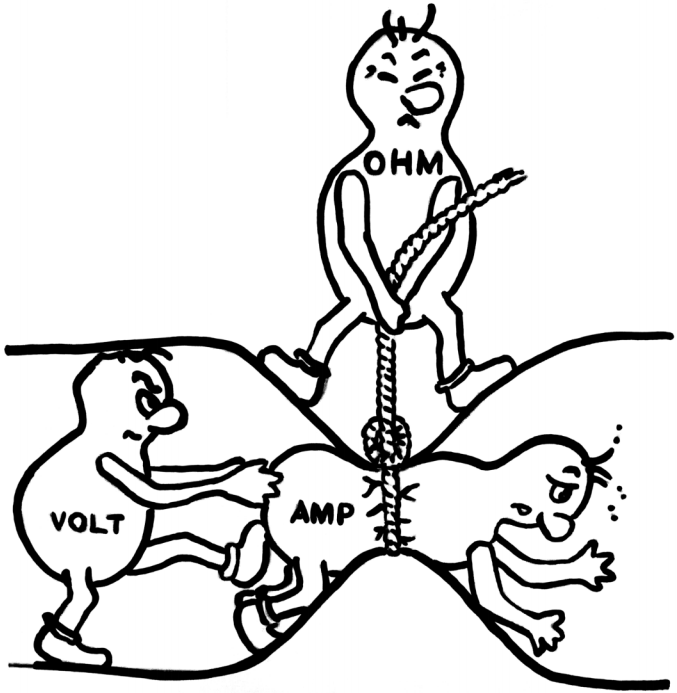
\includegraphics[scale=0.15]{URI.png}
 \vspace{-6cm}
\end{wrapfigure}

\section*{Theorie- und Prüfungsfragen}



%\loesung{
%\begin{figure}[H]
%\centering
%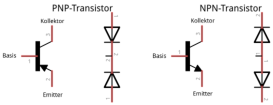
\includegraphics[scale=3]{Transistor/Bilder/PNP_NPN.pdf}
%\caption{1 und 2 - NPN- und PNP-Transistor}
%\end{figure}
%}

% TODO Loesungswege?

\mucho{1}{TB903}
{Welche Spannung lässt einen Strom von $2A$ durch einen Widerstand von $50\Omega$ fließen?}%Frage
{$25V$}%A
{$200V$}%B
{$100V$}%C
{$52V$}%D
{C}%Lösung

\mucho{2}{TD302}
{Die Leerlaufspannung einer Gleichspannungsquelle beträgt $13,5V$. Wenn die Spannungsquelle einen Strom von $1A$ abgibt, sinkt die Klemmenspannung auf $12,4V$. Wie groß ist der Innenwiderstand der Spannungsquelle?}%Frage
{$1,1\Omega$}%A
{$1,2\Omega$}%B
{$12,4\Omega$}%C
{$13,5\Omega$}%D
{A}%Lösung

\mucho{3}{TB908}
{Ein mit einer künstlichen $50\Omega$-Antenne in Serie geschaltetes HF-Amperemeter zeigt $2A$ an. Welche Leistung gibt der Sender ab?}%Frage
{$100W$}%A
{$200W$}%B
{$25\Omega$}%C
{$250\Omega$}%D
{B}%Lösung

\mucho{4}{TB104}
{Welche Gruppe von Materialien enthält nur Nichtleiter?}%Frage
{Pertinax, Polyvinylchlorid (PVC), Graphit}%A
{Epoxid, Polyethylen (PE), Polystyrol (PS)}%B
{Polyethylen (PE), Messing, Konstantan}%C
{Teflon, Pertinax, Bronze}%D
{B}%Lösung

\aufgabentext{
	\begin{enumerate}
	\item[5] \emph{\textbf{TC105-107}} Ordne den folgenden Schaltzeichen die Bezeichnungen LDR, PTC, NTC und VDR zu.\\
		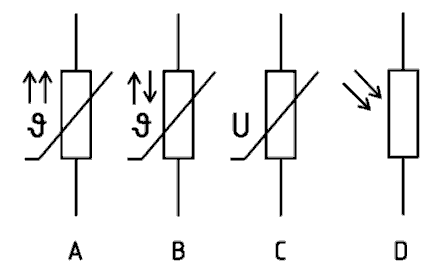
\includegraphics[scale=0.3]{Bild04.png}
		\loesung{Lösung: A PTC, B NTC, C VDR, D LDR}
		\end{enumerate}
	}

\mucho{6}{TC101}
{Die Farbringe gelb, violett und orange auf einem Widerstand mit 4 Farbringen bedeuten einen Widerstandswert von}%Frage
{$4,7k\Omega$}%A
{$47k\Omega$}%B
{$470k\Omega$}%C
{$4,7M\Omega$}%D
{gelb: 4; violett: 7; orange: $\cdot 10^3$; ergibt $47000\Omega$ oder $47k\Omega$: B}%Lösung

\mucho{7}{TC110}
{Welchen Wert hat ein SMD-Widerstand mit der Kennzeichnung 221?}%Frage
{$221\Omega$}%A
{$22k\Omega$}%B
{$22\Omega$}%C
{$220\Omega$}%D
{D}%Lösung

\mucho{8}{TC108}
{Ein Widerstand hat eine Toleranz von $10 \%$. Bei einem nominalen Widerstandswert von $5,6 k\Omega$ liegt der tatsächliche Wert zwischen}%Frage
{$4760$ und $6440 \Omega$}%A
{$5040$ und $6160 \Omega$}%B
{$4,7$ und $6,8 k\Omega$}%C
{$5,2$ und $6,3 k\Omega.$}%D
{B}%Lösung

\mucho{9}{TD108}
{Die Gesamtspannung U an folgendem Spannungsteiler beträgt $12,2V$. Die
Widerstände haben die Werte $R_1 = 10k\Omega$ und $R_2 = 2,2k\Omega$. Wie groß
ist die Teilspannung $U_2$?\\ 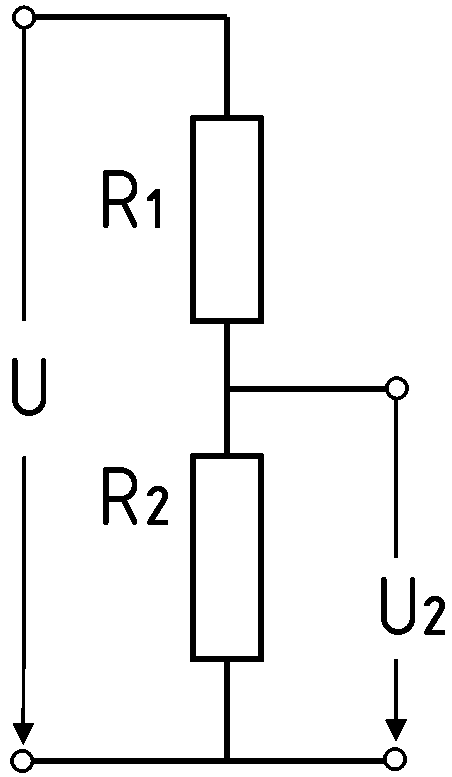
\includegraphics[scale=0.15]{Spannungsteiler.png}}%Frage
{$2,20V$}%A
{$2,64V$}%B
{$10,0V$}%C
{$1,22V$}%D
{A}%Lösung

\mucho{10}{TD103}
{Wie groß ist der Ersatzwiderstand der Gesamtschaltung? 
$R_1 = 500\Omega$, $R_2 = 500\Omega$ und $R_3 = 1k\Omega$\\ 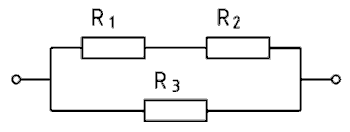
\includegraphics[scale=0.4]{Parallelschaltung.png}}%Frage
{$250\Omega$}%A
{$500\Omega$}%B
{$1k\Omega$}%C
{$2k\Omega$}%D
{B}%Lösung

%----------------------------
\clearpage

\section*{Praktische Anwendung}

\loesung{
    In diesem ersten Praxisteil Elektronik geht es darum die Teilnehmenden mit
    dem Kursmaterial vertraut zu machen und erste Schaltungen zu bauen und zu
    messen. Ablauf:

    \begin{enumerate}
        \item Vorstellung des Kurskofferskonzepts und der Werkzeugtaschen
        \item Grundlagen Breadboard/Messtechnik: U, I, R, P 
    \end{enumerate}

    Besondere Vorbereitungen: \emph{keine}
}

\subsection*{Grundlagen Breadboard/Messtechnik: U, I, R, P}

Material:

\begin{itemize}
    \item Breadboard
    \item Batteriefach
    \item 9V-Blockbatterie
    \item Steckbrücken-/kabel
    \item LED
    \item 2x Widerstand (unbekannt) \loesung{470 $\Omega$ \& 1k $\Omega$}
\end{itemize}

Hinweis: Achtet darauf die Pole des Batteriepacks nicht kurzzuschließen -- wird
sehr heiß und blubbert!

Aufgaben:

% FIXME Platzhalter R1 = ... etc. für die Antworten einfügen, ggf. Schaltplan
% FIXME Tabelle mit 5/6-Ringe-Farbsystem

\begin{enumerate}
  \item Wie ist das Batteriefach aufgebaut und wie verhalten sich Spannung und
    Strom? \\
    \loesung{Spannungen der Zellen addieren sich in Reihe, Strom überall
    gleich}
  \item Ihr habt zwei Widerstände zur Verfügung. Bestimmt die Bauteilwerte
    anhand der Ringe und messt sie nach. \\
    R1 = \dots \loesung{470} $\Omega$ \\
    R2 = \dots \loesung{1k} $\Omega$ \\
    Toleranz: 5\%
  \item Baut einen Stromkreis mit einer LED und den beiden Vorwiderständen
    (einmal seriell, einmal parallel) auf dem Breadboard auf. Was ändert sich?
    Berechnet und messt jeweils den Gesamtvorwiderstand! \\
    \loesung{Parallel: 213 $\Omega$, Serie 1470 $\Omega$}
  \item Verwendet die parallele Gesamtschaltung für die weiteren Messungen
    \begin{enumerate}
      \item Messt die Einzelströme durch die Widerstände! Rechnet nach! \\
        \loesung{Messung: 470 $\Omega$: $\approx$ 20-30mA, 1k $\Omega$: $\approx$ 10 mA, $U_r$ = 6,6 V, $I_{ges}$ = 30 mA}\\
        \loesung{Rechnung: 470 $\Omega$: $\approx$ 14 mA, 1k $\Omega$: $\approx$ 6,6 mA, $I_{ges}$ = 20,6 mA}
      \item Messt die notwendigen Spannungen um die Leistungsaufnahme der
        Gesamtschaltung sowie der LED zu berechnen! Was fällt euch auf? \\
        \loesung{$I_{ges}$ = 30 mA, $U_{ges}$ = 9,11 V, $U_{LED}$ = 2,45 V, $P_{LED}$ = 73 mW, $P_{ges}$ = 273 mW, $\eta$ = 27\%}
    \end{enumerate}
  \item Zusatzaufgabe: Spannungsteiler LED\\

\end{enumerate}

% FIXME Mit Folien von Lars zusammenführen: Zusatzaufgabe Spannungsteiler.
